% !TEX root = saveliev_physics_general_course_2.tex
%!TEX TS-program = pdflatex
%!TEX encoding = UTF-8 Unicode


\chapter[ELECTROMAGNETIC INDUCTION]{ELECTROMAGNETIC\\ INDUCTION}\label{chap:8}
\chaptermark{ELECTROMAGNETIC INDUCTION}

\section{The Phenomenon of Electromagnetic Induction}\label{sec:8_1}

In 1831, the British physicist and chemist Michael Faraday (1791-1867) discovered that an electric current is produced in a closed conducting loop when the flux of magnetic induction through the surface enclosed by this loop changes.
This phenomenon is called \textbf{electromagnetic induction}, and the current produced an \textbf{induced current}.

The phenomenon of electromagnetic induction shows that when the magnetic flux in a loop changes, an induced electromotive force $\ab{\mathcal{E}}{i}$ is set up.
The value of $\ab{\mathcal{E}}{i}$ does not depend on how the magnetic flux $\Phi$ is changed and is determined only by the rate of change of $\Phi$, \ie, by the value of $\diffin{\Phi}{t}$.
A change in the sign of $\diffin{\Phi}{t}$ is attended
by a change in the direction of $\ab{\mathcal{E}}{i}$.

Let us consider the following example.
Figure \ref{fig:8_1} shows loop $1$ whose current $I_1$ can be varied by means of a rheostat.
This current sets up a magnetic field through loop $2$.
If we increase the current $I_1$, the magnetic induction flux $\Phi$ through loop $2$ will grow.
This will lead to the appearance in loop $2$ of the induced current $I_2$ registered by a galvanometer.
Diminishing of the current $I_1$ will cause the magnetic flux through the second loop to decrease.
This will result in the appearance in it of an induced current of a direction opposite to that in the first case.
An induced current $I_2$ can also be set up by bringing loop $2$ closer to loop $1$ or moving it away from it.
In these two cases, the directions of the induced current are opposite.
Finally, electromagnetic induction can be produced without translational motion of loop $2$, but by turning it so as to change the angle between a normal to the loop and the direction of the field.

\begin{figure}[t]
	\begin{center}
		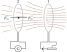
\includegraphics[scale=1]{figures/ch_08/fig_8_1.pdf}
		\caption[]{}
		\label{fig:8_1}
	\end{center}
	\vspace{-0.8cm}
\end{figure}

E. Lenz established a rule permitting us to find the direction of an induced current.
\textbf{Lenz's rule} states that an induced current is always directed so as to oppose the cause producing it.
If, for example, a change in $\Phi$ is due to motion of loop $2$, then an induced current is set up of a direction such that the force of interaction with the first loop opposes the motion of the loop.
When loop $2$ approaches loop $1$ (see \fig{8_1}), a current $I_2'$ is set up whose magnetic moment is directed oppositely to the field of the current $I_1$ (the angle a between the vectors $\ab{\vec{p}}{m}'$ and $\vec{B}$ is $\pi$s).
Hence, loop $2$ will experience a force repelling it from loop $1$ [see \eqn{6_77}].
When loop $2$ is moved away from loop $1$, the current $I_2''$ is produced whose moment $\ab{\vec{p}}{m}''$ coincides in direction with the field of the current $I_1$ ($\alpha=0$) so that the force exerted on loop $2$ is directed toward loop $1$.

Assume that both loops are stationary and the current in loop $2$ is induced by changing the current $I_1$ in loop $1$.
Now a current $I_2$ is induced of a direction such that the intrinsic magnetic flux it produces tends to weaken the change in the external flux leading to the setting up of the induced current.
When $I_1$ grows, \ie, the external magnetic flux directed to the right is increased, a current $I_2'$ is induced that sets up a flux directed to the left.
When $I_1$ diminishes, the current $I_2''$ is set up whose intrinsic magnetic flux has the same direction as the external flux and, consequently, tends to keep the external flux unchanged.

\section{Induced E.M.F.}\label{sec:8_2}

We have established in the preceding section that changes in the magnetic flux $\Phi$ through a loop set up an induced e.m.f. $\ab{\mathcal{E}}{i}$ in it.
To find the relation between $\ab{\mathcal{E}}{i}$ and the rate of change of $\Phi$, we shall consider the following example.

Let us take a loop with a movable rod of length $l$ (\fig{8_2}a).
We shall put it in a homogeneous magnetic field at right angles to the plane of the loop and directed beyond the drawing.
Let us bring the rod into motion with the velocity $\vec{v}$.
The current carriers in the rod---electrons---will also begin to move relative to the field with the same velocity.
As a result, each electron will begin to experience the magnetic force
\begin{equation}\label{eq:8_1}
    \vec{F}_{\parallel} = -e (\vecprod{v}{B}),
\end{equation}

\noindent
directed along the rod [see \eqn{6_33}; the charge of an electron is $-e$].
The action of this force is equivalent to the action on an electron of an electric field of strength
\begin{equation*}
    \vec{E} = \vecprod{v}{B}.
\end{equation*}

\noindent
This field is of a non-electrostatic origin. Its circulation around a loop gives the value of the e.m.f. induced in the loop:
\begin{equation}\label{eq:8_2}
    \ab{\mathcal{E}}{i} = \oint \vec{E} \ccdot \derivec{l} = \oint (\vecprod{v}{B}) \ccdot \derivec{l} = \int_1^2 (\vecprod{v}{B}) \ccdot \derivec{l}
\end{equation}

\noindent
(the integrand differs from zero only on section $1$-$2$ formed by the rod).

To be able to judge about the direction in which the e.m.f. acts according to the sign of $\ab{\mathcal{E}}{i}$, we shall consider $\ab{\mathcal{E}}{i}$ positive when its direction forms a right-handed system with the direction of a normal to the loop.

\begin{figure}[t]
	\begin{center}
		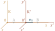
\includegraphics[scale=1]{figures/ch_08/fig_8_2.pdf}
		\caption[]{}
		\label{fig:8_2}
	\end{center}
	\vspace{-0.8cm}
\end{figure}

Let us choose the normal as shown in \fig{8_2}.
Hence, when calculating the circulation, we must circumvent the loop clockwise and choose the direction of the vectors $\derivec{l}$ accordingly.
If we put the constant vector $\vecprod{v}{B}$ in \eqn{8_2} outside the integral, we get
\begin{equation*}
    \ab{\mathcal{E}}{i} = (\vecprod{v}{B}) \int_1^2 \derivec{l} = (\vecprod{v}{B}) \ccdot \vec{l},
\end{equation*}

\noindent
where $\vec{l}$ is the vector depicted in \fig{8_2}b.
Let us perform a cyclic rearrangement of the multipliers in the expression obtained, after which we shall multiply and divide it by $\deriv{t}$:
\begin{equation}\label{eq:8_3}
    \ab{\mathcal{E}}{i} = \vec{B} \ccdot (\vecprod{l}{v}) = \frac{\vec{B} \ccdot (\vec{l} \times \vec{v}\, \deriv{t})}{\deriv{t}}.
\end{equation}

\noindent
A glance at \fig{8_2}b shows that
\begin{equation*}
    \vec{l} \times \vec{v}\, \deriv{t} = - \hatvec{n}\, \deriv{S},
\end{equation*}

\noindent
where $\deriv{S}$ is the increment of the loop area during the time $\deriv{t}$.
By the definition of a flux, $\vec{B}\ccdot{\derivec{S}}=\vec{B}\ccdot\hatvec{n}\,\deriv{S}$ is the flux through the area $\deriv{S}$, \ie, the increment of the flux $\deriv{\Phi}$ through the loop.
Thus,
\begin{equation*}
    \vec{B} \ccdot (\vec{l} \times \vec{v}\, \deriv{t}) = - \vec{B} \ccdot \hatvec{n}\, \deriv{S} = - \deriv{\Phi}.
\end{equation*}

\noindent
With a view to this expression, \eqn{8_3} can be written as
\begin{equation}\label{eq:8_4}
    \ab{\mathcal{E}}{i} = - \diff{\Phi}{t}.
\end{equation}

We have found that $\diffin{\Phi}{t}$ and $\ab{\mathcal{E}}{i}$ have opposite signs.
The sign of the flux and that of $\ab{\mathcal{E}}{i}$ are associated with the choice of the direction of a normal to the plane of a loop.
With our selection of the normal (see \fig{8_2}), the sign of $\diffin{\Phi}{t}$ is positive, and that of $\ab{\mathcal{E}}{i}$ is negative.
If we had chosen a normal directed not beyond the drawing, but toward us, the sign of $\diffin{\Phi}{t}$ would be negative and that of It
positive.

The SI unit of magnetic induction flux is the \textbf{weber} (\si{\weber}), which is the flux through a surface of \SI{1}{\metre\squared} intersected by magnetic field lines normal to it with $B = \SI{1}{\tesla}$.
At a rate of change of the flux equal to \SI{1}{\weber\per\second}, an e.m.f. of \SI{1}{\volt} is induced in the loop.
In the Gaussian system of units, \eqn{8_4} has the form
\begin{equation}\label{eq:8_5}
    \ab{\mathcal{E}}{i} = - \frac{1}{c} \diff{\Phi}{t}.
\end{equation}

\noindent
The unit of $\Phi$ in this system is the \textbf{maxwell} (\si{\maxwell}) equal to the flux through a surface of \SI{1}{\centi\metre\squared} at $B = \SI{1}{\gauss}$.
Equation \eqref{eq:8_5} gives $\ab{\mathcal{E}}{i}$
in cgse$_U$.
To find it in volts, we must multiply the result obtained by $300$. Since $300/c = \num{e-8}$, we have
\begin{equation}\label{eq:8_6}
    \ab{\mathcal{E}}{i}(V) = -\num{e-8}\, \diff{\Phi}{t} \parenthesis{\si{\maxwell\per\second}}.
\end{equation}

In the reasoning that led us to \eqn{8_4}, the part of the extraneous forces maintaining a current in a loop was played by magnetic forces.
The work of these forces on a unit positive charge, equal by definition to the e.m.f., is other than zero.
This circumstance apparently contradicts the statement made in \sect{6_5} that a magnetic force can do no work on a charge.
This contradiction is eliminated if we take into account that the force \eqref{eq:8_1} is not the total magnetic force exerted on an electron, but only the component of this force parallel to the conductor and due to the velocity $\vec{v}$ (see the force $\vec{F}_{\parallel}$ in \fig{8_3}).
This component causes the electron to start moving along the conductor with the velocity $\vec{u}$, as a result of which a magnetic force perpendicular to the wire is set up equal to
\begin{equation*}
    \vec{F}_{\parallel} = - e (\vecprod{u}{B})
\end{equation*}

\noindent
(this component makes no contribution to the circulation because it is perpendicular to $\derivec{l}$).

\begin{figure}[t]
	\begin{center}
		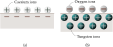
\includegraphics[scale=1]{figures/ch_08/fig_8_3.pdf}
		\caption[]{}
		\label{fig:8_3}
	\end{center}
	\vspace{-0.8cm}
\end{figure}

The total magnetic force exerted on an electron is
\begin{equation*}
    \vec{F} = \vec{F}_{\parallel} + \vec{F}_{\perp},
\end{equation*}

\noindent
and the work of this force on an electron during the time $\deriv{t}$ is
\begin{equation*}
    \deriv{A} = \vec{F}_{\parallel} \ccdot \vec{u}\, \deriv{t} + \vec{F}_{\perp} \ccdot \vec{v}\, \deriv{t} = F_{\parallel} u\, \deriv{t} + F_{\perp} v\, \deriv{t}
\end{equation*}

\noindent
(the directions of the vectors $\vec{F}_{\parallel}$ and $\vec{u}$ are the same, and of the vectors $\vec{F}_{\perp}$ and $\vec{v}$ are opposite; see \fig{8_3}).
Substituting for the magnitudes of the forces their values $F_{\parallel}=evB$ and $F_{\perp}=euB$, we find that the work of the total magnetic force equals zero.

The force $\vec{F}_{\perp}$ is directed oppositely to the velocity of the rod $\vec{v}$.
Therefore, for the rod to move with the constant velocity $\vec{v}$, the external force $\ab{\vec{F}}{ext}$ must be applied to it that balances the sum of the forces $\vec{F}_{\perp}$ applied to all the electrons contained in the rod.
It is exactly at the expense of the work of this force that the energy liberated in the loop by the induced current will be produced.

Our explanation of the appearance of an induced e.m.f. relates to the case when the magnetic field is constant, while the geometry of the loop changes.
The magnetic flux through the loop can also be changed, however, by changing $\vec{B}$.
In this case, the explanation of the appearance of an e.m.f. will differ in principle.
The time-varying magnetic field sets up a vortex electric field $\vec{E}$ (this is treated in detail in \sect{9_1}).
The action of the field $\vec{E}$ causes the current carriers in a conductor to start moving---an induced current is set up.
The relation between the induced e.m.f. and the changes in the magnetic flux in this case too is described by \eqn{8_4}.

Assume that the loop in which an e.m.f. is induced consists of $N$ turns instead of one, \ie, it is a solenoid, for example.
Since the turns are connected in series, $\ab{\mathcal{E}}{i}$ will equal the sum of the e. m.f.'s induced in each of the turns separately:
\begin{equation*}
    \ab{\mathcal{E}}{i} = - \sum \diff{\Phi}{t} = - \diff{}{t}\parenthesis{\sum \Phi}.
\end{equation*}

The quantity
\begin{equation}\label{eq:8_7}
    \Psi = \sum \Phi,
\end{equation}

\noindent
is called the \textbf{flux linkage} or the \textbf{total magnetic flux}. It is measured in the same units as $\Phi$.
If the flux through each of the turns is the same, then
\begin{equation}\label{eq:8_8}
    \Psi = N \Phi.
\end{equation}

\noindent
The e.m.f. induced in an intricate loop is determined by the formula
\begin{equation}\label{eq:8_9}
    \ab{\mathcal{E}}{i} = - \diff{\Psi}{t}.
\end{equation}

\section{Ways of Measuring the Magnetic Induction}\label{sec:8_3}

Assume that the total magnetic flux linked to a loop changes from $\Psi_1$ to $\Psi_2$.
Let us find the charge $q$ that flows through each section of the loop.
The instantaneous value of the current in the loop is
\begin{equation*}
	I = \frac{\mathcal{E}}{R} = - \frac{1}{R} \diff{\Psi}{t}.
\end{equation*}

\noindent
Hence,
\begin{equation*}
	\deriv{q} = I\, \deriv{t} = - \frac{1}{R} \diff{\Psi}{t}\, \deriv{t} = - \frac{1}{R}\, \deriv{\Psi}.
\end{equation*}

\noindent
Integration of this expression yields the total charge:
\begin{equation}\label{eq:8_10}
	q = \int \deriv{q} = - \frac{1}{R} \int_1^2 \deriv{\Psi} = \frac{1}{R} (\Psi_1 - \Psi_2).
\end{equation}

Equation \eqref{eq:8_10} underlies the ballistic method of measuring the magnetic induction developed by A. Stoletov.
It consists in the following.
A small coil with $N$ turns is placed in the field being studied.
The coil is arranged so that the vector $\vec{B}$ is perpendicular to the plane of the turns (\fig{8_4}a).
Hence, the total magnetic flux linked with the coil will be
\begin{equation*}
	\Psi_1 = NBS,
\end{equation*}

\noindent
where $S$ is the area of one turn, which must be so small that the field within its limits may be considered homogeneous.

\begin{figure}[t]
	\begin{center}
		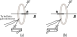
\includegraphics[scale=1]{figures/ch_08/fig_8_4.pdf}
		\caption[]{}
		\label{fig:8_4}
	\end{center}
	\vspace{-0.8cm}
\end{figure}

When the coil is turned through $180$ degrees (\fig{8_4}b), the flux linkage becomes equal to $\Psi_2=-NBS$ ($\hatvec{n}$ and $\vec{B}$ are directed oppositely).
Hence, the change in the total flux linkage when the coil is turned is $\Psi_1 - \Psi_2 = 2NBS$. If the coil is turned sufficiently quickly, a short current pulse is produced in the loop upon which the charge
\begin{equation}\label{eq:8_11}
	q = \frac{1}{R} 2NBS
\end{equation}

\noindent
flows [see \eqn{8_10}].

The charge flowing in the circuit during the short current pulse can be measured with the aid of a so-called \textbf{ballistic galvanometer}.
The latter is a galvanometer with a great period of natural oscillations.
Having measured $q$ and knowing $R$, $N$, and $S$, we can find $B$ by \eqn{8_11}.
By $R$, here, is meant the resistance of the entire circuit including the coil, the connecting wires, and the galvanometer.

Instead of turning the coil, we may switch on (or off) the magnetic field being studied, or reverse its direction.

To measure $B$, the circumstance is also used that the electric resistance of bismuth grows greatly under the action of a magnetic field---by about five per cent per tenth of a tesla (per \SI{1000}{\gauss}).
Consequently, we can determine the magnetic induction of a magnetic field by placing a preliminarily graduated bismuth coil (\fig{8_5}) into the field and measuring the relative change in its resistance.

We must note that the electric resistance of other metals also grows in a magnetic field, but to a much smaller extent.
For copper, for example, the increase in the resistance is about one-ten thousandth of that for bismuth.

\section{Eddy Currents}\label{sec:8_4}

Induced currents can also be produced in solid massive conductors.
In this case, they are known as \textbf{eddy currents}.
The electric resistance of a massive conductor is small, therefore, the eddy currents may reach a very high value.

\begin{figure}[t]
	\begin{minipage}[t]{0.48\linewidth}
		\begin{center}
			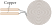
\includegraphics[scale=1]{figures/ch_08/fig_8_5.pdf}
			\caption[]{}
			\label{fig:8_5}
		\end{center}
	\end{minipage}
	\hfill{ }%space{-0.05cm}
	\begin{minipage}[t]{0.48\linewidth}
		\begin{center}
			
\includegraphics[scale=1]{figures/ch_08/fig_8_6.pdf}
			\caption[]{}
			\label{fig:8_6}
		\end{center}
	\end{minipage}
\vspace{-0.4cm}
\end{figure}

In accordance with Lenz's rule, eddy currents choose paths and directions in a conductor such as to resist by their action the reason setting them up as much as possible.
This is why good conductors moving in a strong magnetic field experience great retardation due to the interaction of the eddy currents with the magnetic field.
This is taken advantage of for damping the movable parts of galvanometers, seismographs, and other instruments.
A conducting (for example, aluminium) plate in the form of a sector is fastened to the movable part of an instrument (\fig{8_6}) and is introduced into the gap between the poles of a strong permanent magnet.
Movement of the plate causes eddy currents to be produced in it that brake the system.
The advantage of such a device is that the braking action appears only when the plate moves and vanishes when the plate is stationary.
Therefore, the electromagnetic damper is absolutely no hindrance to the instrument accurately arriving at its equilibrium position.

The thermal action of eddy currents is used in induction furnaces.
Such a furnace is a coil supplied with a high-frequency current of a high value.
If we place a conducting body inside the coil, intensive eddy currents will be produced in it that
can heat the body up to its melting point.
This method is used to melt metals in vacuum.
The resulting materials have an exceedingly high purity.

Eddy currents are also used to heat the internal metal components of vacuum installations in order to degas them.

Eddy currents are quite often undesirable, and special measures must be taken to eliminate them.
For example, to prevent the losses of energy for heating transformer cores by eddy currents, the cores are assembled of thin insulated sheets.
The latter are arranged so that the possible directions of the eddy currents will be perpendicular to them.
The appearance of ferrites (semiconductor magnetic materials with a high electric resistance) made it possible to manufacture solid cores.

The eddy currents set up in conductors carrying alternating currents are directed so as to weaken the current inside a conductor and increase it near the surface.
As a result, the fast-varying current is distributed
unevenly over the cross section of the conductor---it is forced out, as it were, to the surface of the conductor.
This phenomenon is called the \textbf{skin effect}.
Owing to this effect, the internal part of conductors in high-frequency circuits is useless. This is why the conductors used for such circuits have the form of tubes.

\section{Self-Induction}\label{sec:8_5}

An electric current flowing in any loop produces the magnetic flux $\Psi$ through this loop.
When $I$ changes, $\Psi$ also changes, and the result
is the induction of an e.m.f. in the loop.
This phenomenon is called \textbf{self-induction}.
In accordance with the Biot-Savart law, the magnetic induction $B$ is proportional to the current setting up the field.
Hence, it follows that the current $I$ in a loop and the total magnetic flux $\Psi$ through the loop it produces are proportional to each other:
\begin{equation}\label{eq:8_12}
	\Psi = L I.
\end{equation}

\noindent
The constant of proportionality $L$ between the current and the total magnetic flux is called the \textbf{inductance} of a loop.

A linear dependence of $\Psi$ on $I$ is observed only if the permeability $\mu$ of the medium surrounding the loop does not depend on the field
strength $H$, \ie, in the absence of ferromagnetics.
Otherwise, $\mu$ is an intricate function of $I$ (through $H$, see \fig{7_19}b), and, since $B=\mu_0\mu H$, the dependence of $\Psi$ on $I$ will also be quite intricate.
Equation \eqref{eq:8_12}, however, is also extended to this case, and the inductance $L$ is considered as a function of $I$.
With a constant current $I$, the total flux $\Psi$ can change as a result of changes in the shape and dimensions of a loop.

It can be seen from the above that the inductance $L$ depends on the geometry of a loop (\ie, on its shape and dimensions), and also on the magnetic properties (on $\mu$) of the medium surrounding the loop.
If the loop is rigid and there are no ferromagnetics near it, the inductance $L$ is a constant quantity.
The SI unit of inductance is the inductance of a conductor in which a total flux $\Psi$ of \SI{1}{\weber} linked with it is set up at a current of \SI{1}{\ampere} in the conductor. This unit is called the \textbf{henry} (\si{\henry}).

In the Gaussian system of units, the inductance has the dimension of length.
Accordingly, the unit of inductance in this system is
called the \textbf{centimetre}.
A loop with which a flux of \SI{1}{\maxwell} (\SI{e-8
}{\weber}) is linked at a current of \SI{1}{\cgs{m}{I}} (\ie, \SI{10}{\ampere}) has an inductance of \SI{1}{\centi\metre}.

Let us calculate the inductance of a solenoid.
We shall take a solenoid so long that it can virtually be considered infinite.
When a current $I$ flows in it, a homogeneous field is produced inside the solenoid whose induction is $B=\mu_0\mu nI$ [see \eqns{6_108}{7_26}].
The flux through each of the turns is $\Phi=BS$, and the total magnetic flux linked with the solenoid is
\begin{equation}\label{eq:8_13}
	\Psi = N\Phi = nlBS = \mu_0 \mu n^2 l S I,
\end{equation}

\noindent
where $l$ is the length of the solenoid (which is assumed to be very great), $S$ is the cross-sectional area, and $n$ the number of turns per unit length (the product $nl$ gives the total number of turns $N$).

A comparison of \eqns{8_12}{8_13} gives the following expression for the inductance of a very long solenoid:
\begin{equation}\label{eq:8_14}
	L = \mu_0 \mu n^2 l S = \mu_0 \mu n^2 V,
\end{equation}

\noindent
where $V = lS$ is the volume of the solenoid.

It follows from \eqn{8_14} that the dimension of $\mu_0$ equals that of inductance divided by the dimension of length.
Accordingly, $\mu_0$ is measured in henry per metre [see \eqn{6_3}].

When the current in a loop changes, a self-induced e.m.f. $\ab{\mathcal{E}}{s}$ is set up that equals
\vspace{-12pt}
\begin{equation}\label{eq:8_15}
	\ab{\mathcal{E}}{s} = - \diff{\Psi}{t} = - \diff{(LI)}{t} = - \parenthesis{L\, \diff{I}{t} + I\, \diff{L}{t}}.
\end{equation}

\noindent
If the inductance remains constant when the current changes (which is possible only in the absence of ferromagnetics), the expression for the self-induced e.m.f. becomes
\begin{equation}\label{eq:8_16}
	\ab{\mathcal{E}}{s} = - L\, \diff{I}{t}.
\end{equation}

\noindent
The minus sign in \eqn{8_16} is due to Lenz's rule according to which an induced current is directed so as to oppose the cause producing it.
In the case being considered, what sets up $\ab{\mathcal{E}}{s}$ is the change of the current in the circuit.
Let us assume clockwise circumvention to be the positive direction.
In these conditions, the current will be greater than zero if it flows clockwise in the circuit and less than zero if it flows counterclockwise.
Similarly, $\ab{\mathcal{E}}{s}$ will be greater than
zero if it is exerted in a clockwise direction, and less than zero if it is exerted in a counterclockwise one.

The derivative $\diffin{I}{t}$ is positive in two cases---either upon a growth in a positive current or upon a decrease in the absolute value of a negative current.
Inspection of \eqn{8_16} shows that in these cases $\ab{\mathcal{E}}{s}<0$.
This signifies that the self-induced e.m.f. is directed counterclockwise and, therefore, is opposed to the above current changes (a growth in a positive or a decrease in a negative current).

The derivative $\diffin{I}{t}$ is negative also in two cases---either when a positive current diminishes, or when the magnitude of a negative current grows. In these cases, $\ab{\mathcal{E}}{s}>0$ and, consequently, opposes changes in the current (a decrease in a positive or a growth in the
magnitude of a negative current).

Equation \eqref{eq:8_16} makes it possible to define the inductance as a constant of proportionality between the rate of change of the current in a loop and the resulting self-induced e.m.f..
Such a definition is lawful, however, only when $L=\text{constant}$.
In the presence of ferromagnetics, $L$ of an undeforming loop will be a function of $I$ (through $H$).
Hence, $\diffin{L}{t}$ can be written as $(\diffin{L}{I})(\diffin{I}{t})$.
Making such a substitution in \eqn{8_15}, we get
\begin{equation}\label{eq:8_17}
	\ab{\mathcal{E}}{s} = - \parenthesis{L + I\, \diff{L}{I}}\, \diff{I}{t}.
\end{equation}

\noindent
We can, thus, see that in the presence of ferromagnetics the constant of proportionality between $\diffin{I}{t}$ and $\ab{\mathcal{E}}{s}$ does not at all equal $L$.

\section{Current When a Circuit Is Opened or Closed}\label{sec:8_6}

According to Lenz's rule, the additional currents set up owing to self-induction are always directed so as to prevent any changes in the current in a circuit.
The result is that a current grows to its steady value when a circuit is closed or drops to zero when the circuit is opened not instantaneously, but gradually.

Let us first find how a current changes when the switch of a circuit is opened.
Assume that a current source of e.m.f. $\mathcal{E}$ is connected in a circuit with an inductance $L$ not depending on $I$ and a resistance $R$ (\fig{8_7}).
The steady current flowing in the circuit will be
\begin{equation}\label{eq:8_18}
	I_0 = \frac{\mathcal{E}}{R}
\end{equation}

\noindent
(we consider the resistance of the current source to
be negligibly small).

\begin{figure}[t]
	\begin{center}
		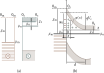
\includegraphics[scale=1]{figures/ch_08/fig_8_7.pdf}
		\caption[]{}
		\label{fig:8_7}
	\end{center}
	\vspace{-0.8cm}
\end{figure}

At the moment $t=0$, let us switch off the current source and simultaneously short the circuit by means of switch SW.
As soon as the current in the circuit begins to diminish, a self-inductance e.m.f. opposing this decrease appears.
The current in the circuit will comply with the equation
\begin{equation*}
	IR = \ab{\mathcal{E}}{s} = - L \diff{I}{t},
\end{equation*}

\noindent
or
\begin{equation}\label{eq:8_19}
	\diff{I}{t} + \frac{R}{L} I = 0.
\end{equation}

\noindent
Equation \eqref{eq:8_19} is a linear homogeneous differential equation of the first order.
Separating variables, we get
\begin{equation*}
	\frac{\deriv{I}}{I} = - \frac{R}{L}\, \deriv{t},
\end{equation*}

\noindent
whence
\begin{equation*}
	\ln{I} = - \frac{R}{L} t + \ln(\text{constant})
\end{equation*}

\noindent
(with a view to further transformations, we have written the integration constant in the form ``$\ln(\text{constant})$'').
Converting this relation to a power yields
\begin{equation}\label{eq:8_20}
	I = \text{constant} \times \exp\parenthesis{- \frac{R}{L} t}.
\end{equation}

\noindent
Equation \eqref{eq:8_20} is a general solution of \eqn{8_19}.
We shall find the value of the constant from the initial conditions.
When $t=0$, the current had the value given by \eqn{8_18}.
Hence, $\text{constant}=I_0$.
Introducing this value into \eqn{8_20}, we arrive at the expression
\begin{equation}\label{eq:8_21}
	I = I_0\, \exp\parenthesis{- \frac{R}{L} t}.
\end{equation}

Thus, after the e.m.f. source had been switched off, the current in the circuit did not vanish instantaneously, but diminished according to the exponential law \eqref{eq:8_21}.
A plot of the diminishing of $I$ is given in \fig{8_8} (curve $1$).
The rate of diminishing is determined by the quantity
\begin{equation}\label{eq:8_22}
	\tau = \frac{L}{R},
\end{equation}

\noindent
having the dimension of time and called the \textbf{time constant} of the circuit.
Substituting $1/\tau$ for $R/L$ in \eqn{8_21}, we get
\begin{equation}\label{eq:8_23}
	I = I_0\, \exp\parenthesis{- \frac{t}{\tau}}.
\end{equation}

\begin{figure}[t]
	\begin{center}
		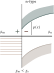
\includegraphics[scale=1]{figures/ch_08/fig_8_8.pdf}
		\caption[]{}
		\label{fig:8_8}
	\end{center}
	\vspace{-0.8cm}
\end{figure}

\noindent
According to this equation, $\tau$ is the time during which the current diminishes to $1/e$-th of its initial value.
A glance at \eqn{8_22} shows that the time constant $\tau$ grows and the current in the circuit diminishes at a slower rate with an increasing inductance $L$ and a decreasing resistance $R$ of the circuit.

To simplify our calculations, we considered that the circuit is shorted when the current source is switched off.
If we simply break a circuit with a high inductance, the high induced voltage set up produces a spark or an arc at the place of breaking of the circuit.

Now let us consider the closing of a circuit.
After the e.m.f. source is switched on, a self-induced e.m.f. will act in the circuit apart from the e.m.f. $\mathcal{E}$ until the current reaches its steady value given by \eqn{8_18}.
Hence, in accordance with Ohm's law
\begin{equation*}
	IR = \mathcal{E} + \ab{\mathcal{E}}{s} + \mathcal{E} - L\, \diff{I}{t},
\end{equation*}

\noindent
or
\begin{equation}\label{eq:8_24}
	\diff{I}{t} + \frac{R}{L} I = \frac{\mathcal{E}}{L}.
\end{equation}

We have arrived at a linear inhomogeneous differential equation that differs from \eqn{8_19} only in that the right-hand side contains the constant quantity $\mathcal{E}/L$ instead of zero.
It is known from the theory of differential equations that the general solution of a linear inhomogeneous equation can be obtained by adding any partial solution of it to the general solution of the corresponding homogeneous equation (see Sec. 7.4 of Vol. I).
The general solution of our homogeneous equation has the form of \eqn{8_20}.
It is easy to see that $I=\mathcal{E}/R=I_0$ is a partial solution of \eqn{8_24}.
Hence, the function
\begin{equation*}
	I = I_0 + \text{constant} \times \exp\parenthesis{- \frac{R}{L} t},
\end{equation*}

\noindent
will be the general solution of \eqn{8_24}.
At the initial moment, the current is zero.
Thus, $\text{constant}=-I_0$, and
\begin{equation}\label{eq:8_25}
	I = I_0 \bracket{1 - \exp\parenthesis{ -\frac{R}{L} t}}.
\end{equation}

\noindent
This function describes the growth of the current in a circuit after a source of an e.m.f. has been switched on in it.
A plot of function \eqref{eq:8_25} is shown in \fig{8_8} (curve $2$).

\section{Mutual Induction}\label{sec:8_7}

Let us take two loops $1$ and $2$ close to each other (\fig{8_9}).
If the current $I_1$ flows in loop $1$, it sets up through loop $2$ a total magnetic flux proportional to $I_1$, \ie,
\begin{equation}\label{eq:8_26}
	\Psi_2 = L_{21} I_1
\end{equation}

\noindent
(the field producing this flux is depicted in the figure by solid lines).
When the current $I_1$ changes, the e.m.f.
\begin{equation}\label{eq:8_27}
	\ab{\mathcal{E}}{i,$2$} = - L_{21}\, \diff{I_1}{t},
\end{equation}

\noindent
is induced in loop $2$ (we assume that there are no ferromagnetics near the loops).

\begin{figure}[t]
	\begin{center}
		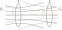
\includegraphics[scale=1]{figures/ch_08/fig_8_9.pdf}
		\caption[]{}
		\label{fig:8_9}
	\end{center}
	\vspace{-0.8cm}
\end{figure}

Similarly, when the current $I_2$ flows in loop $2$, the following flux linked with loop $1$ appears:
\begin{equation}\label{eq:8_28}
	\Psi_1 = L_{12} I_2
\end{equation}

\noindent
(the field producing this flux is depicted in the figure by dash lines).
When the current $I_2$ changes, the e.m.f.
\begin{equation}\label{eq:8_29}
	\ab{\mathcal{E}}{i,$1$} = - L_{12}\, \diff{I_2}{t},
\end{equation}

\noindent
is induced in loop $1$.

Loops $1$ and $2$ are called \textbf{coupled}, while the phenomenon of the setting up of an e.m.f. in one of the loops upon changes in the current in the other is called \textbf{mutual induction}.

The coefficients of proportionality $L_{12}$ and $L_{21}$ are called the \textbf{mutual inductances} of the loops.
The relevant calculations show that in the absence of ferromagnetics these coefficients are always equal to each other:
\begin{equation}\label{eq:8_30}
	L_{12} = L_{21}.
\end{equation}

\noindent
Their magnitude depends on the shape, dimensions,
and mutual arrangement of the loops, and also on the permeability of the medium surrounding the loops.
The quantity $L_{12}$ is measured in the same units as the inductance $L$.

Let us find the mutual inductance of two coils wound onto a common toroidal iron core (\fig{8_10}).
The magnetic induction lines are concentrated inside the core [see the text following \eqn{7_31}].
We can, therefore, consider that the magnetic field set up by any of the windings will have the same strength throughout the core.
If the first winding has $N_1$ turns and the current $I_1$ flows through it, then according to the theorem on circulation [see \eqn{7_11}], we have
\begin{equation}\label{eq:8_31}
	Hl = N_1 I_1
\end{equation}

\noindent
(here, $l$ is the length of the core).

\begin{figure}[t]
	\begin{center}
		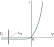
\includegraphics[scale=1]{figures/ch_08/fig_8_10.pdf}
		\caption[]{}
		\label{fig:8_10}
	\end{center}
	\vspace{-0.8cm}
\end{figure}

The magnetic flux through the cross section of the core is $\Phi=BS=\mu_0\mu HS$, where $S$ is the cross-sectional area of the core.
Introducing the value of $H$ from \eqn{8_31} and multiplying the expression obtained by $N_2$, we get the total flux linked with the second winding:
\begin{equation*}
	\Psi_2 = \frac{S}{l} \mu_0 \mu N_1 N_2 I_1.
\end{equation*}

\noindent
A comparison of this equation with \eqn{8_26} shows that
\begin{equation}\label{eq:8_32}
	L_{21} = \frac{S}{l} \mu_0 \mu N_1 N_2.
\end{equation}

Calculations of the flux $\Psi_1$ linked with the first winding when the current $I_2$ flows through the second winding yields the equation
\begin{equation}\label{eq:8_33}
	L_{12} = \frac{S}{l} \mu_0 \mu N_1 N_2,
\end{equation}

\noindent
which coincides in form with $L_{21}$ [see \eqn{8_31}].
In the given case, however, we cannot assert that $L_{12}=L_{21}$. The factor $\mu$ in the expressions for these coefficients depends on the field strength $H$ in the core.
If $N_1\neq N_2$, then the same current passed once through the first winding and another time through the second one will set up a field of different strength $H$ in the core.
Accordingly, the values of $\mu$ in both cases will be different so that when $I_1=I_2$ the numerical values of $L_{12}$ and $L_{21}$ do not coincide.

\section{Energy of a Magnetic Field}\label{sec:8_8}

Let us consider the circuit shown in \fig{8_11}.
When the switch is closed, the current $I$ will be set up in the solenoid.
It will produce a magnetic field linked with the solenoid turns.
If the switch is opened, a gradually diminishing current will flow for a certain time through resistor $R$.
This current is maintained by the self-induced e.m.f. produced in the solenoid.
The work done by the current during the time $\deriv{t}$ is
\begin{equation}\label{eq:8_34}
	\deriv{A} = \ab{\mathcal{E}}{s} I\, \deriv{t} = -\diff{\Psi}{t} I\, \deriv{t} = -I\, \deriv{\Psi}.
\end{equation}

\begin{figure}[t]
	\begin{center}
		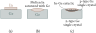
\includegraphics[scale=0.95]{figures/ch_08/fig_8_11.pdf}
		\caption[]{}
		\label{fig:8_11}
	\end{center}
	\vspace{-0.8cm}
\end{figure}

If the inductance of the solenoid does not depend on $I$ ($L=\text{constant}$), then $\deriv{\Psi}=L\,\deriv{I}$, and \eqn{8_34} becomes
\begin{equation}\label{eq:8_35}
	\deriv{A} = - LI\, \deriv{I}.
\end{equation}

\noindent
Integrating this expression with respect to $I$ within the limits from the initial value of $I$ to zero, we get the work done in the circuit during the entire time needed for vanishing of the magnetic field:
\begin{equation}\label{eq:8_36}
	A = - \int_I^0 LI\, \deriv{I} = \frac{LI^2}{2}.
\end{equation}

The work \eqref{eq:8_36} is spent on an increment of the internal energy of the resistor $R$, the solenoid, and the connecting wires (\ie, on heating them).
This work is attended by vanishing of the magnetic field that initially existed in the space surrounding the solenoid.
Since no other changes occur in the bodies surrounding the circuit, it remains for us to conclude that the magnetic field is a carrier of energy, and it is exactly at the expense of the latter that the work given by \eqn{8_36} is done.
We, thus, arrive at the conclusion that a conductor of inductance $L$ carrying the current $I$ has the energy
\begin{equation}\label{eq:8_37}
	W = \frac{LI^2}{2},
\end{equation}

\noindent
that is localized in the magnetic field set up by the current [compare this equation with the expression $CU^2/2$ for the energy of a charged capacitor; see \eqn{4_5}].

Equation \eqref{eq:8_36} can be interpreted as the work that must be done against the self-induced e.m.f. when the current grows from $0$ to $I$, and that is used to set up a magnetic field having the energy given by \eqn{8_37}.
Indeed, the work done against the self-induced e.m.f. is
\begin{equation*}
	A' = \int_0^I (-\ab{\mathcal{E}}{s}) I\, \deriv{t}.
\end{equation*}

\noindent
Performing transformations similar to those which led us to \eqn{8_35}, we get
\begin{equation}\label{eq:8_38}
	A' = \int_0^I LI\, \deriv{I} = \frac{LI^2}{2},
\end{equation}

\noindent
that coincides with \eqn{8_36}.
The work according to \eqn{8_38} is done when the current sets in at the expense of the e.m.f. source.
It is used completely for producing a magnetic field linked with the solenoid turns.
Equation \eqref{eq:8_38} takes no account of the work
spent by the e.m.f. source for heating the conductors during the time the current reaches its steady value.

Let us express the energy of a magnetic field given by \eqn{8_37} through quantities characterizing the field itself.
For a long (virtually infinite) solenoid
\begin{equation*}
	L = \mu_0\mu n^2V,\quad H=nI,\quad\text{or}\quad I=\frac{H}{n}
\end{equation*}

\noindent
[see \eqns{7_29}{8_14}].
Using these values of $L$ and $I$ in \eqn{8_37} and performing the relevant transformations, we obtain
\begin{equation}\label{eq:8_39}
	W = \frac{\mu_0 \mu H^2}{2} V.
\end{equation}

It was shown in \sect{6_12} that the magnetic field of an infinitely long solenoid is homogeneous and differs from zero only inside the solenoid.
Hence, the energy according to \eqn{8_39} is localized inside the solenoid and is distributed over its volume with a constant density $w$ that can be found by dividing $W$ by $V$.
This division yields
\begin{equation}\label{eq:8_40}
	w = \frac{\mu_0 \mu H^2}{2}.
\end{equation}

\noindent
Using \eqn{7_17}, we can write the equation for the energy density of a magnetic field as follows:
\begin{equation}\label{eq:8_41}
	w = \frac{\mu_0 \mu H^2}{2} = \frac{HB}{2} = \frac{B^2}{2 \mu_0 \mu}.
\end{equation}

The expressions we have obtained for the energy density of a magnetic field differ from Eqs. \eqref{eq:4_11} for the energy density of an electric field only in that the electrical quantities in them have been replaced with the relevant magnetic ones.

Knowing the density of the field energy at every point, we can find the energy of the field enclosed in any volume $V$.
For this purpose, we must calculate the integral
\begin{equation}\label{eq:8_42}
	W = \int_V w\, \deriv{V} = \int_V \frac{\mu_0 \mu H^2}{2}\, \deriv{V}.
\end{equation}

It can be shown that for coupled loops (in the absence of ferromagnetics) the field energy is determined by the equation
\begin{equation}\label{eq:8_43}
	W = \frac{L_1 I_1^2}{2} + \frac{L_2 I_2^2}{2} + \frac{L_{12} I_1 I_2}{2} + \frac{L_{21} I_2 I_1}{2}.
\end{equation}

\noindent
A similar expression is obtained for the energy of $N$ loops coupled to one another:
\begin{equation}\label{eq:8_44}
	W = \frac{1}{2} \sum_{i,k=1}^N L_{i,k} I_i I_k,
\end{equation}

\noindent
where $L_{i,k}=L_{k,i}$ is the mutual inductance of the $i$-th and $k$-th loops, and $L_{i,i}=L_i$ is the inductance of the $i$-th loop.

\section{Work in Magnetic Reversal of a Ferromagnetic}\label{sec:8_9}

Changes in a current in a circuit are attended by the performance of work against the self-induced e.m.f.:
\begin{equation}\label{eq:8_45}
	\derivp{A} = (-\ab{\mathcal{E}}{s}) I\, \deriv{t} = \diff{\Psi}{t} I\, \deriv{t} = I\, \deriv{\Psi}.
\end{equation}

\noindent
If the inductance of the circuit $L$ remains constant (which is possible only in the absence of ferromagnetics), this work is used completely for producing the energy of a magnetic field: $\derivp{A}=\deriv{W}$.
We shall now see that matters are different when ferromagnetics are present.

For a very long (``infinite'') solenoid, $H=nI$, $\Psi=nlBS$.
Hence,
\begin{equation*}
	I = \frac{H}{n},\quad \deriv{\Psi} = nlS\, \deriv{B}.
\end{equation*}

\noindent
Introducing these expressions into \eqn{8_45}, we get
\begin{equation}\label{eq:8_46}
	\derivp{A} = H\, \deriv{B} \times V,
\end{equation}

\noindent
where $V=lS$ is the volume of the solenoid, \ie, the volume in which a homogeneous magnetic feild has been produced.

Let us see whether we can identify \eqn{8_46} with the increment of the energy of a magnetic field.
We remind our reader that energy is a function of state.
Therefore, the sum of its increments for a cyclic process is zero:
\begin{equation*}
	\oint \deriv{W} = 0.
\end{equation*}

\noindent
If we fill a solenoid with a ferromagnetic, then the relation between $B$ and $H$ is depicted by the curve shown in \fig{8_12}.
The expression $H\,\deriv{B}$ gives the area of the shaded strip.
Consequently, the integral $\oint H\,\deriv{B}$ calculated along the hysteresis loop equals the area $S_l$ enclosed by the loop.
Thus, the integral of expression \eqref{eq:8_46}, \ie, $\oint\derivp{A}$, differs from zero.
It, therefore, follows that in the presence of ferromagnetics, the work given by \eqn{8_46} cannot
be equated to the increment of the energy of a magnetic field.
Upon completion of the cycle of magnetic reversal, $H$ and $B$ and, therefore, the magnetic energy will have their initial values.
Hence, the work $\oint\derivp{A}$ is not used to produce the energy of a magnetic field.
Experiments show that it is used to increase the internal energy of the ferromagnetic, \ie, to heat it.

\begin{figure}[t]
	\begin{center}
		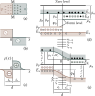
\includegraphics[scale=1]{figures/ch_08/fig_8_12.pdf}
		\caption[]{}
		\label{fig:8_12}
	\end{center}
	\vspace{-0.8cm}
\end{figure}

Thus, the completion of one cycle of magnetic reversal of a ferromagnetic is attended by the expenditure of work per unit volume numerically equal to the area of the hysteresis loop:
\begin{equation}\label{eq:8_47}
	\ab{A}{u.vol} = \oint H\, \deriv{B} = S_l.
\end{equation}

\noindent
This work goes to heat the ferromagnetic.

In the absence of ferromagnetics, $B$ is an unambiguous function of $H$ ($B=\mu_0\mu H$, where $\mu=\text{constant}$).
Therefore, the expression $H\,\deriv{B}=\mu_0\mu H\, \deriv{H}$ is a total differential
\begin{equation}\label{eq:8_48}
	\deriv{w} = H\,\deriv{B},
\end{equation}

\noindent
determining the increment of the energy of a magnetic field.
Integration of \eqn{8_48} within the limits from $0$ to $H$ leads to \eqn{8_40} for the density of the field energy (before performing integration, $H\,\deriv{B}$ must be transformed by substituting $\mu_0\mu\,\deriv{H}$ for $\deriv{B}$).
